
%%%%%%%%%%%%%%%%%% PREAMBULE %%%%%%%%%%%%%%%%%%

\documentclass[aspectratio=169,utf8]{beamer}
%\documentclass[aspectratio=169,handout]{beamer}

\usetheme{Boadilla}
%\usecolortheme{seahorse}
%\usecolortheme[RGB={245,66,24}]{structure}
\useoutertheme{infolines}

% packages
\usepackage{amsfonts,amsmath,amssymb,amsthm}
\usepackage[utf8]{inputenc}
\usepackage[T1]{fontenc}
\usepackage{lmodern}

\usepackage[francais]{babel}
\usepackage{fancybox}
\usepackage{graphicx}

\usepackage{float}
\usepackage{xfrac}

%\usepackage[usenames, x11names]{xcolor}
\usepackage{pgfplots}
\usepackage{datetime}


% ----------------------------------------------------------------------
% Pour les images
\usepackage{tikz}
\usetikzlibrary{calc,shadows,arrows.meta,patterns,matrix}

\newcommand{\tikzinput}[1]{\input{figures/#1.tikz}}
% --- les figures avec échelle éventuel
\newcommand{\myfigure}[2]{% entrée : échelle, fichier(s) figure à inclure
\begin{center}\small%
\tikzstyle{every picture}=[scale=1.0*#1]% mise en échelle + 0% (automatiquement annulé à la fin du groupe)
#2%
\end{center}}



%-----  Package unités -----
\usepackage{siunitx}
\sisetup{locale = FR,detect-all,per-mode = symbol}

%\usepackage{mathptmx}
%\usepackage{fouriernc}
%\usepackage{newcent}
%\usepackage[mathcal,mathbf]{euler}

%\usepackage{palatino}
%\usepackage{newcent}
% \usepackage[mathcal,mathbf]{euler}



% \usepackage{hyperref}
% \hypersetup{colorlinks=true, linkcolor=blue, urlcolor=blue,
% pdftitle={Exo7 - Exercices de mathématiques}, pdfauthor={Exo7}}


%section
% \usepackage{sectsty}
% \allsectionsfont{\bf}
%\sectionfont{\color{Tomato3}\upshape\selectfont}
%\subsectionfont{\color{Tomato4}\upshape\selectfont}

%----- Ensembles : entiers, reels, complexes -----
\newcommand{\Nn}{\mathbb{N}} \newcommand{\N}{\mathbb{N}}
\newcommand{\Zz}{\mathbb{Z}} \newcommand{\Z}{\mathbb{Z}}
\newcommand{\Qq}{\mathbb{Q}} \newcommand{\Q}{\mathbb{Q}}
\newcommand{\Rr}{\mathbb{R}} \newcommand{\R}{\mathbb{R}}
\newcommand{\Cc}{\mathbb{C}} 
\newcommand{\Kk}{\mathbb{K}} \newcommand{\K}{\mathbb{K}}

%----- Modifications de symboles -----
\renewcommand{\epsilon}{\varepsilon}
\renewcommand{\Re}{\mathop{\text{Re}}\nolimits}
\renewcommand{\Im}{\mathop{\text{Im}}\nolimits}
%\newcommand{\llbracket}{\left[\kern-0.15em\left[}
%\newcommand{\rrbracket}{\right]\kern-0.15em\right]}

\renewcommand{\ge}{\geqslant}
\renewcommand{\geq}{\geqslant}
\renewcommand{\le}{\leqslant}
\renewcommand{\leq}{\leqslant}
\renewcommand{\epsilon}{\varepsilon}

%----- Fonctions usuelles -----
\newcommand{\ch}{\mathop{\text{ch}}\nolimits}
\newcommand{\sh}{\mathop{\text{sh}}\nolimits}
\renewcommand{\tanh}{\mathop{\text{th}}\nolimits}
\newcommand{\cotan}{\mathop{\text{cotan}}\nolimits}
\newcommand{\Arcsin}{\mathop{\text{arcsin}}\nolimits}
\newcommand{\Arccos}{\mathop{\text{arccos}}\nolimits}
\newcommand{\Arctan}{\mathop{\text{arctan}}\nolimits}
\newcommand{\Argsh}{\mathop{\text{argsh}}\nolimits}
\newcommand{\Argch}{\mathop{\text{argch}}\nolimits}
\newcommand{\Argth}{\mathop{\text{argth}}\nolimits}
\newcommand{\pgcd}{\mathop{\text{pgcd}}\nolimits} 


%----- Commandes divers ------
\newcommand{\ii}{\mathrm{i}}
\newcommand{\dd}{\text{d}}
\newcommand{\id}{\mathop{\text{id}}\nolimits}
\newcommand{\Ker}{\mathop{\text{Ker}}\nolimits}
\newcommand{\Card}{\mathop{\text{Card}}\nolimits}
\newcommand{\Vect}{\mathop{\text{Vect}}\nolimits}
\newcommand{\Mat}{\mathop{\text{Mat}}\nolimits}
\newcommand{\rg}{\mathop{\text{rg}}\nolimits}
\newcommand{\tr}{\mathop{\text{tr}}\nolimits}


%----- Structure des exercices ------

\newtheoremstyle{styleexo}% name
{2ex}% Space above
{3ex}% Space below
{}% Body font
{}% Indent amount 1
{\bfseries} % Theorem head font
{}% Punctuation after theorem head
{\newline}% Space after theorem head 2
{}% Theorem head spec (can be left empty, meaning ‘normal’)

%\theoremstyle{styleexo}
\newtheorem{exo}{Exercice}
\newtheorem{ind}{Indications}
\newtheorem{cor}{Correction}


\newcommand{\exercice}[1]{} \newcommand{\finexercice}{}
%\newcommand{\exercice}[1]{{\tiny\texttt{#1}}\vspace{-2ex}} % pour afficher le numero absolu, l'auteur...
\newcommand{\enonce}{\begin{exo}} \newcommand{\finenonce}{\end{exo}}
\newcommand{\indication}{\begin{ind}} \newcommand{\finindication}{\end{ind}}
\newcommand{\correction}{\begin{cor}} \newcommand{\fincorrection}{\end{cor}}

\newcommand{\noindication}{\stepcounter{ind}}
\newcommand{\nocorrection}{\stepcounter{cor}}

\newcommand{\fiche}[1]{} \newcommand{\finfiche}{}
\newcommand{\titre}[1]{\centerline{\large \bf #1}}
\newcommand{\addcommand}[1]{}
\newcommand{\video}[1]{}

% Marge
\newcommand{\mymargin}[1]{\marginpar{{\small #1}}}

\def\noqed{\renewcommand{\qedsymbol}{}}


%----- Presentation ------
\setlength{\parindent}{0cm}

%\newcommand{\ExoSept}{\href{http://exo7.emath.fr}{\textbf{\textsf{Exo7}}}}

\definecolor{myred}{rgb}{0.93,0.26,0}
\definecolor{myorange}{rgb}{0.97,0.58,0}
\definecolor{myyellow}{rgb}{1,0.86,0}

\newcommand{\LogoExoSept}[1]{  % input : echelle
{\usefont{U}{cmss}{bx}{n}
\begin{tikzpicture}[scale=0.1*#1,transform shape]
  \fill[color=myorange] (0,0)--(4,0)--(4,-4)--(0,-4)--cycle;
  \fill[color=myred] (0,0)--(0,3)--(-3,3)--(-3,0)--cycle;
  \fill[color=myyellow] (4,0)--(7,4)--(3,7)--(0,3)--cycle;
  \node[scale=5] at (3.5,3.5) {Exo7};
\end{tikzpicture}}
}


\newcommand{\debutmontitre}{
  \author{} \date{} 
  \thispagestyle{empty}
  \hspace*{-10ex}
  \begin{minipage}{\textwidth}
    \titlepage  
  \vspace*{-2.5cm}
  \begin{center}
    \LogoExoSept{2.5}
  \end{center}
  \end{minipage}

  \vspace*{-0cm}
  
  % Astuce pour que le background ne soit pas discrétisé lors de la conversion pdf -> png
\begin{tikzpicture}
        \fill[opacity=0,green!60!black] (0,0)--++(0,0)--++(0,0)--++(0,0)--cycle; 
\end{tikzpicture}

% toc S'affiche trop tot :
% \tableofcontents[hideallsubsections, pausesections]
}

\newcommand{\finmontitre}{
  \end{frame}
  \setcounter{framenumber}{0}
} % ne marche pas pour une raison obscure

%----- Commandes supplementaires ------

% \usepackage[landscape]{geometry}
% \geometry{top=1cm, bottom=3cm, left=2cm, right=10cm, marginparsep=1cm
% }
% \usepackage[a4paper]{geometry}
% \geometry{top=2cm, bottom=2cm, left=2cm, right=2cm, marginparsep=1cm
% }

%\usepackage{standalone}


% New command Arnaud -- november 2011
\setbeamersize{text margin left=24ex}
% si vous modifier cette valeur il faut aussi
% modifier le decalage du titre pour compenser
% (ex : ici =+10ex, titre =-5ex

\theoremstyle{definition}
%\newtheorem{proposition}{Proposition}
%\newtheorem{exemple}{Exemple}
%\newtheorem{theoreme}{Théorème}
%\newtheorem{lemme}{Lemme}
%\newtheorem{corollaire}{Corollaire}
%\newtheorem*{remarque*}{Remarque}
%\newtheorem*{miniexercice}{Mini-exercices}
%\newtheorem{definition}{Définition}

% Commande tikz
\usetikzlibrary{calc}
\usetikzlibrary{patterns,arrows}
\usetikzlibrary{matrix}
\usetikzlibrary{fadings} 

%definition d'un terme
\newcommand{\defi}[1]{{\color{myorange}\textbf{\emph{#1}}}}
\newcommand{\evidence}[1]{{\color{blue}\textbf{\emph{#1}}}}
\newcommand{\assertion}[1]{\emph{\og#1\fg}}  % pour chapitre logique
%\renewcommand{\contentsname}{Sommaire}
\renewcommand{\contentsname}{}
\setcounter{tocdepth}{2}



%------ Encadrement ------

\usepackage{fancybox}


\newcommand{\mybox}[1]{
\setlength{\fboxsep}{7pt}
\begin{center}
\shadowbox{#1}
\end{center}}

\newcommand{\myboxinline}[1]{
\setlength{\fboxsep}{5pt}
\raisebox{-10pt}{
\shadowbox{#1}
}
}

%--------------- Commande beamer---------------
\newcommand{\beameronly}[1]{#1} % permet de mettre des pause dans beamer pas dans poly


\setbeamertemplate{navigation symbols}{}
\setbeamertemplate{footline}  % tiré du fichier beamerouterinfolines.sty
{
  \leavevmode%
  \hbox{%
  \begin{beamercolorbox}[wd=.333333\paperwidth,ht=2.25ex,dp=1ex,center]{author in head/foot}%
    % \usebeamerfont{author in head/foot}\insertshortauthor%~~(\insertshortinstitute)
    \usebeamerfont{section in head/foot}{\bf\insertshorttitle}
  \end{beamercolorbox}%
  \begin{beamercolorbox}[wd=.333333\paperwidth,ht=2.25ex,dp=1ex,center]{title in head/foot}%
    \usebeamerfont{section in head/foot}{\bf\insertsectionhead}
  \end{beamercolorbox}%
  \begin{beamercolorbox}[wd=.333333\paperwidth,ht=2.25ex,dp=1ex,right]{date in head/foot}%
    % \usebeamerfont{date in head/foot}\insertshortdate{}\hspace*{2em}
    \insertframenumber{} / \inserttotalframenumber\hspace*{2ex} 
  \end{beamercolorbox}}%
  \vskip0pt%
}


\definecolor{mygrey}{rgb}{0.5,0.5,0.5}
\setlength{\parindent}{0cm}
%\DeclareTextFontCommand{\helvetica}{\fontfamily{phv}\selectfont}

% background beamer
\definecolor{couleurhaut}{rgb}{0.85,0.9,1}  % creme
\definecolor{couleurmilieu}{rgb}{1,1,1}  % vert pale
\definecolor{couleurbas}{rgb}{0.85,0.9,1}  % blanc
\setbeamertemplate{background canvas}[vertical shading]%
[top=couleurhaut,middle=couleurmilieu,midpoint=0.4,bottom=couleurbas] 
%[top=fondtitre!05,bottom=fondtitre!60]



\makeatletter
\setbeamertemplate{theorem begin}
{%
  \begin{\inserttheoremblockenv}
  {%
    \inserttheoremheadfont
    \inserttheoremname
    \inserttheoremnumber
    \ifx\inserttheoremaddition\@empty\else\ (\inserttheoremaddition)\fi%
    \inserttheorempunctuation
  }%
}
\setbeamertemplate{theorem end}{\end{\inserttheoremblockenv}}

\newenvironment{theoreme}[1][]{%
   \setbeamercolor{block title}{fg=structure,bg=structure!40}
   \setbeamercolor{block body}{fg=black,bg=structure!10}
   \begin{block}{{\bf Th\'eor\`eme }#1}
}{%
   \end{block}%
}


\newenvironment{proposition}[1][]{%
   \setbeamercolor{block title}{fg=structure,bg=structure!40}
   \setbeamercolor{block body}{fg=black,bg=structure!10}
   \begin{block}{{\bf Proposition }#1}
}{%
   \end{block}%
}

\newenvironment{corollaire}[1][]{%
   \setbeamercolor{block title}{fg=structure,bg=structure!40}
   \setbeamercolor{block body}{fg=black,bg=structure!10}
   \begin{block}{{\bf Corollaire }#1}
}{%
   \end{block}%
}

\newenvironment{mydefinition}[1][]{%
   \setbeamercolor{block title}{fg=structure,bg=structure!40}
   \setbeamercolor{block body}{fg=black,bg=structure!10}
   \begin{block}{{\bf Définition} #1}
}{%
   \end{block}%
}

\newenvironment{lemme}[0]{%
   \setbeamercolor{block title}{fg=structure,bg=structure!40}
   \setbeamercolor{block body}{fg=black,bg=structure!10}
   \begin{block}{\bf Lemme}
}{%
   \end{block}%
}

\newenvironment{remarque}[1][]{%
   \setbeamercolor{block title}{fg=black,bg=structure!20}
   \setbeamercolor{block body}{fg=black,bg=structure!5}
   \begin{block}{Remarque #1}
}{%
   \end{block}%
}


\newenvironment{exemple}[1][]{%
   \setbeamercolor{block title}{fg=black,bg=structure!20}
   \setbeamercolor{block body}{fg=black,bg=structure!5}
   \begin{block}{{\bf Exemple }#1}
}{%
   \end{block}%
}


\newenvironment{miniexercice}[0]{%
   \setbeamercolor{block title}{fg=structure,bg=structure!20}
   \setbeamercolor{block body}{fg=black,bg=structure!5}
   \begin{block}{Mini-exercices}
}{%
   \end{block}%
}


\newenvironment{tp}[0]{%
   \setbeamercolor{block title}{fg=structure,bg=structure!40}
   \setbeamercolor{block body}{fg=black,bg=structure!10}
   \begin{block}{\bf Travaux pratiques}
}{%
   \end{block}%
}
\newenvironment{exercicecours}[1][]{%
   \setbeamercolor{block title}{fg=structure,bg=structure!40}
   \setbeamercolor{block body}{fg=black,bg=structure!10}
   \begin{block}{{\bf Exercice }#1}
}{%
   \end{block}%
}
\newenvironment{algo}[1][]{%
   \setbeamercolor{block title}{fg=structure,bg=structure!40}
   \setbeamercolor{block body}{fg=black,bg=structure!10}
   \begin{block}{{\bf Algorithme}\hfill{\color{gray}\texttt{#1}}}
}{%
   \end{block}%
}


\setbeamertemplate{proof begin}{
   \setbeamercolor{block title}{fg=black,bg=structure!20}
   \setbeamercolor{block body}{fg=black,bg=structure!5}
   \begin{block}{{\footnotesize Démonstration}}
   \footnotesize
   \smallskip}
\setbeamertemplate{proof end}{%
   \end{block}}
\setbeamertemplate{qed symbol}{\openbox}


\makeatother
\usecolortheme[RGB={192,41,0}]{structure}

% Commande spécifique à ce chapitre

\newcommand{\Python}{\texttt{Python}}
\renewcommand{\evidence}[1]{{\color{blue}\textbf{#1}}}

\usepackage{textcomp}

\usepackage{listings}
\lstset{
  upquote=true,
  columns=flexible,
  keepspaces=true,
  basicstyle=\ttfamily,
  commentstyle=\color{gray},
  language=Python,
  showstringspaces=false,
  aboveskip=0em,  
  belowskip=0em,
  escapeinside=||
}

\lstset{
  literate={é}{{\'e}}1
           {è}{{\`e}}1
           {à}{{\`a}}1
}


\newcommand{\codeinline}[1]{\lstinline!#1!}


%%%%%%%%%%%%%%%%%%%%%%%%%%%%%%%%%%%%%%%%%%%%%%%%%%%%%%%%%%%%%
%%%%%%%%%%%%%%%%%%%%%%%%%%%%%%%%%%%%%%%%%%%%%%%%%%%%%%%%%%%%%


\begin{document}


\title{{\bf Algorithmes et mathématiques}}
\subtitle{Arithmétique -- Algorithmes récursifs}

\begin{frame}
  
  \debutmontitre

  \pause

{\footnotesize
\hfill
\setbeamercovered{transparent=50}
\begin{minipage}{0.6\textwidth}
  \begin{itemize}
    \item<3-> Algorithmes récursifs
    \item<4-> L'algorithme d'Euclide
    \item<5-> Nombres premiers
  \end{itemize}
\end{minipage}
}

\end{frame}

\setcounter{framenumber}{0}


%%%%%%%%%%%%%%%%%%%%%%%%%%%%%%%%%%%%%%%%%%%%%%%%%%%%%%%%%%%%%%%%
\section{Algorithmes récursifs}


\begin{frame}[fragile]

\begin{algo}[iteratif.py]
\begin{lstlisting}
def factorielle_classique(n):
    produit = 1
    for i in range(1,n+1):
        produit = i * produit
    return produit
\end{lstlisting}  
\end{algo}

\pause
\bigskip

\codeinline{factorielle_classique(5)}

\pause

\codeinline{produit = 1}
\pause

\codeinline{produit = 1 * produit = 1}

\pause

\codeinline{produit = 2 * produit = 2}

\pause

\codeinline{produit = 3 * produit = 6}

\pause

\codeinline{produit = 4 * produit = 24}

\pause

\codeinline{produit = 5 * produit = 120 } \pause \codeinline{ = 5!}

\end{frame}


\begin{frame}[fragile]

\begin{algo}[recursif.py (1)]
\begin{lstlisting}
def factorielle(n):
    if (n==1): 
        return 1
    else:
        return n * factorielle(n-1)
\end{lstlisting}  
\end{algo}

\pause
\bigskip

\codeinline{factorielle(5)}

\pause

\codeinline{factorielle(5) = 5 * factorielle(4)}

\pause

\codeinline{factorielle(5) = 5 * 4 * factorielle(3)}

\pause

\codeinline{factorielle(5) = 5 * 4 * 3 * factorielle(2)}

\pause

\codeinline{factorielle(5) = 5 * 4 * 3 * 2 *  factorielle(1)}

\pause

\codeinline{factorielle(5) = 5 * 4 * 3 * 2 * 1 }\pause\ \codeinline{ = 5!}

\end{frame}


\begin{frame}[fragile]

\begin{itemize}
  \item Une \defi{fonction récursive} est une fonction qui 
  s'appelle elle-même lorsque elle s’exécute 
\pause  
  \item Analogie avec la récurrence
\pause  
  \item $u_n = n!$ \pause \hfill $u_1 = 1 \quad \text{ et } \quad u_{n} = n \times u_{n-1} \text{ si } n \ge 2$
\pause  
  \item 
  \begin{itemize}
    \item \evidence{initialisation} \pause \qquad  \codeinline{if (n==1): return 1}
\pause 
    \item \evidence{hérédité} \pause \qquad\qquad  \codeinline{return n * factorielle(n-1)}
  \end{itemize}  
\end{itemize}
\end{frame}


\begin{frame}[fragile]

\hfill\hfill\textbf{Nombres de Fibonacci}

$$1 \quad 1 \quad 2 \quad 3 \quad 5 \quad 8 \quad 13 \quad 21 \quad 34 \quad \ldots$$

\pause

$$F_0 = 1, \ F_1 = 1 \quad \text{ et } \quad F_{n} = F_{n-1} + F_{n-2} \quad  \text{ si } n \ge 2$$

\pause


\begin{algo}[recursif.py (2)]
\begin{lstlisting}
def fibonacci(n):
    if (n==0) or (n==1):
        return 1           |\pause|
    else: 
        return fibonacci(n-1)+fibonacci(n-2)
\end{lstlisting}  
\end{algo}

\end{frame}




%%%%%%%%%%%%%%%%%%%%%%%%%%%%%%%%%%%%%%%%%%%%%%%%%%%%%%%%%%%%%%%%
\section{L'algorithme d'Euclide}

\begin{frame}

\hfill\hfill\textbf{Algorithme d'Euclide}

$$\text{si } b | a \text{ alors } \pgcd(a,b)=b  \qquad \text{ sinon } \pgcd(a,b) = \pgcd(b, a \bmod b)$$

\pause

\begin{tp}
\begin{enumerate}
  \item Créer une fonction récursive \codeinline{pgcd(a,b)} qui calcule le pgcd.
  \item On note $p_n$ la probabilité que deux entiers $a,b$ tirés au hasard dans 
  ${1,2,\ldots,n}$ soient premiers entre eux. Faire une fonction qui approxime $p_n$.
  Lorsque $n$ devient grand, comparer $p_n$ et $\frac{6}{\pi^2}$.
\end{enumerate}  
\end{tp}

\end{frame}


\begin{frame}[fragile]

\begin{algo}[arith.py (1)]
\begin{lstlisting}
def pgcd(a,b):
    if a%b == 0:
        return b    |\pause|
    else:
        return pgcd(b, a%b)
\end{lstlisting}  
\end{algo}
\end{frame}

\begin{frame}[fragile]

\centerline{$a,b$ sont \defi{premiers entre eux} si $\pgcd(a,b)=1$}

\pause

\begin{algo}[arith.py (2)]
\small
\begin{lstlisting}
def nb_premiers_entre_eux(n,nbtirages):
    i = 1
    nbpremiers = 0
    while i <= nbtirages:
        i = i+1
        a = random.randint(1,n)
        b = random.randint(1,n)
        if pgcd(a,b)==1:
            nbpremiers = nbpremiers + 1
    return nbpremiers
\end{lstlisting}  
\end{algo}

\pause

\begin{itemize}
  \item Exemple : $n=1000$, $10\,000$ tirages $1 \le a,b \le 1000$
\pause  
  \item Probabilité \codeinline{nbpremiers/nbtirages} $\simeq 0,60\ldots$
\pause  
  \item $n$ tend vers $+\infty$ alors $p_n \to \frac{6}{\pi^2} = 0,607927\ldots$ 
\pause  
  \item \og La probabilité que deux entiers tirés au hasard soient premiers entre eux est $\frac{6}{\pi^2}$ \fg
\end{itemize}

\end{frame}


\begin{frame}

Commentaires sur les algorithmes récursifs
\pause
\begin{itemize}
  \item 
  \begin{itemize}
    \item Code très court
\pause
    \item Proche de la formulation mathématique d'une récurrence
  \end{itemize}
 \pause 
  
  \item Il peut y avoir des problèmes de mémoire
 \pause 
  
  \item Bien poser la condition initiale
 \pause 
  \item Il n'existe pas des algorithmes récursifs pour tout !
\end{itemize}

\end{frame}


%%%%%%%%%%%%%%%%%%%%%%%%%%%%%%%%%%%%%%%%%%%%%%%%%%%%%%%%%%%%%%%%
\section{Nombres premiers}


\begin{frame}

\begin{tp}
\begin{enumerate}
  \item \'Ecrire une fonction qui détecte si un nombre $n$ est premier ou pas en testant s'il existe des entiers 
  $k$ qui divise $n$. (On se limitera aux entiers $2 \le k \le \sqrt{n}$, pourquoi ?).
  \item Faire un algorithme pour le crible d'Eratosthène : écrire tous les entiers de $2$ à $n$,
  conserver $2$ (qui est premier) et barrer tous les multiples suivants de $2$. Le premier nombre non barré (c'est $3$) est premier.
  Barrer tous les multiples suivants de $3$,...
  \item Dessiner la spirale d'Ulam : on place les nombres entiers en spirale, et on colorie en rouge les nombres premiers.
  $$\begin{matrix} & & \cdots & \cdots \\ 5 & 4 & 3 & \vdots \\ 6 & 1 & 2 & 11 \\ 7 & 8 & 9 & 10 \\\end{matrix}$$
\end{enumerate}  
\end{tp}

\end{frame}

\begin{frame}[fragile]

\begin{algo}[arith.py (3)]
\begin{lstlisting}
def est_premier(n):
    if (n<=1): return False  |\pause|
    k = 2
    while k*k <= n:
        if n%k==0:            
            return False     |\pause|
        else: 
            k = k +1         |\pause|
    return True              
\end{lstlisting}  
\end{algo}

\pause

\begin{itemize}
  \item $n$ n'est pas premier alors $n=a\times b$ avec $a,b \ge 2$
\pause  
  \item $a \le \sqrt n$ ou $b \le \sqrt n$ \pause : il suffit de tester les diviseurs $2 \le k \le \sqrt{n}$
\pause  
  \item \codeinline{k*k <= n} \pause plus rapide que \codeinline{k <= sqrt(n)}
 \pause 
  \item \defi{Booléen} est une variable qui vaut soit Vrai, soit Faux 
\end{itemize}

 
\end{frame}



\begin{frame}[fragile]

\begin{algo}[arith.py (4)]{\small
\begin{lstlisting}
def eratosthene(n):
    liste_entiers = list(range(n+1))     # tous les entiers  |\pause|
    liste_entiers[1] = 0              # 1 n'est pas premier  |\pause|
    k = 2                                  # multiples de 2  
    while k*k <= n:                                      
        if liste_entiers[k] != 0:    # si k n'est pas barré  
            i = k                         # i multiple de k
            while i <= n-k:
                i = i+k
                liste_entiers[i] = 0    # barrer mult. de k  
        k = k +1                                          |\pause| 
    liste_premiers = [k for k in liste_entiers if k !=0]
    return liste_premiers
\end{lstlisting}  }
\end{algo}

\pause

\codeinline{[0,0,2,3,4,5,6,7,8,9,10,11,12,13,...]}

\pause

\codeinline{[0,0,2,3,0,5,0,7,0,9,0,11,0,13,...]}

\pause

\codeinline{[0,0,2,3,0,5,0,7,0,0,0,11,0,13,...]}

\pause

\codeinline{[2,3,5,7,11,13,...]}

\end{frame}


\begin{frame}

\hfill\hfill\textbf{Spirale d'Ulam}

\bigskip

\begin{center}
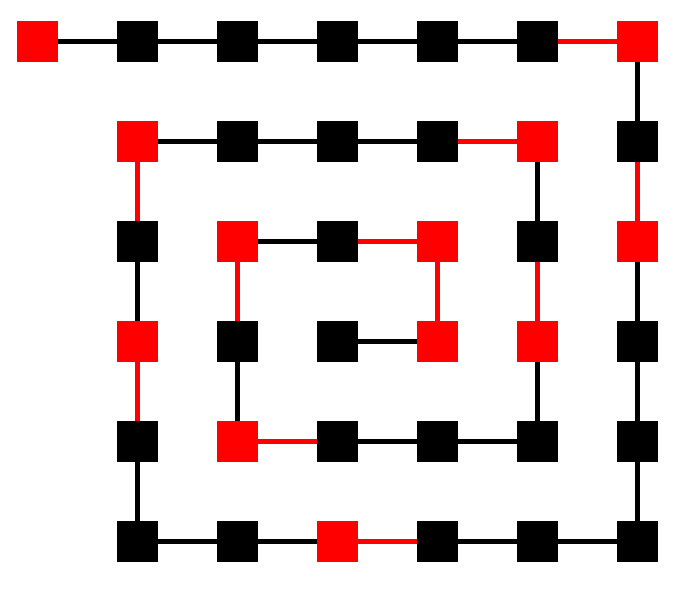
\includegraphics[scale=0.23]{figures/ulam1}
\qquad \pause
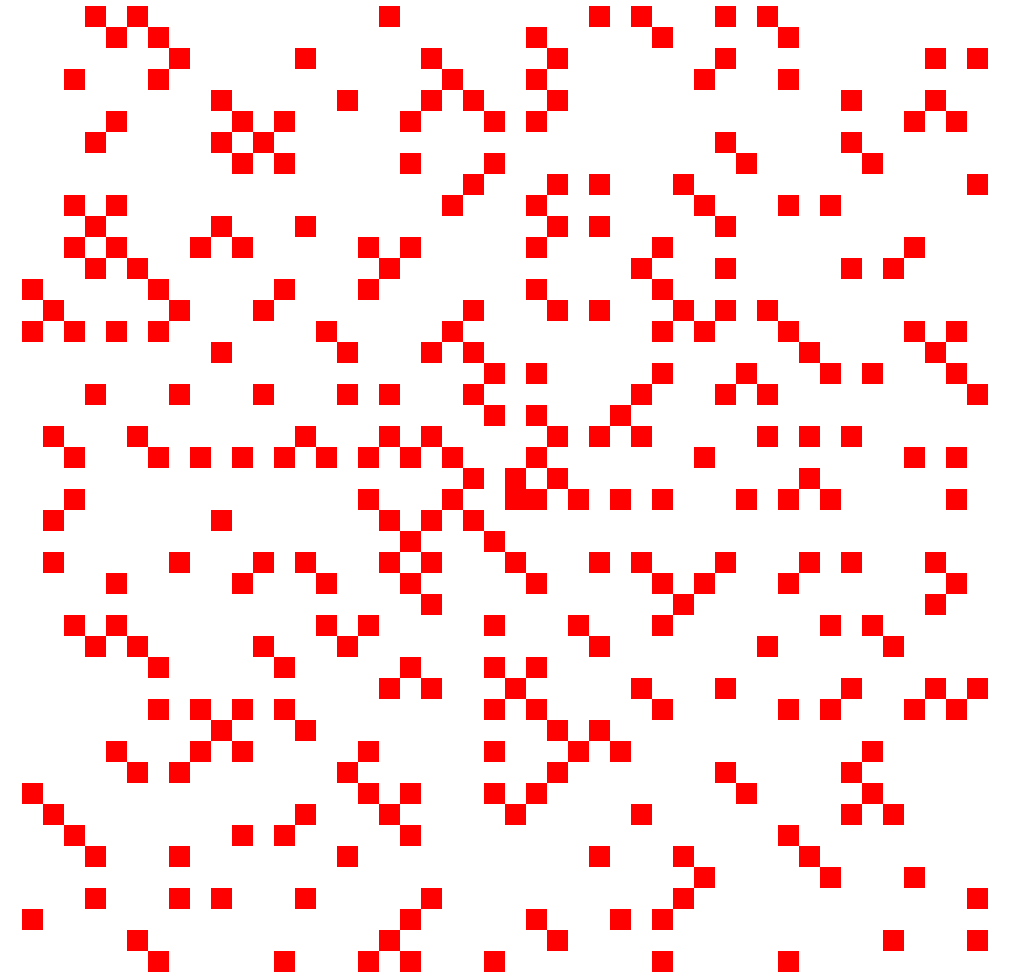
\includegraphics[scale=0.14]{figures/ulam2}
\end{center}

\end{frame}




%%%%%%%%%%%%%%%%%%%%%%%%%%%%%%%%%%%%%%%%%%%%%%%%%%%%%%%%%%%%%%%%
\section{Mini-exercices}

\begin{frame}
\small\vspace*{-1ex}
\begin{miniexercice}
\vspace*{-1ex}
\begin{enumerate}
\setlength{\itemsep}{0pt}
  \item \'Ecrire une version itérative et une version récursive pour les fonctions suivantes : 
  (a) la somme des carrés des entiers de $1$ à $n$ ; 
  (b) $2^n$ (sans utiliser d'exposant) ;
  (c) la partie entière d'un réel $x\ge0$ ;
  (d) le quotient de la division euclidienne de $a$ par $b$ (avec $a \in \Nn$, $b \in \Nn^*$) ;
  (e) le reste de cette division euclidienne (sans utiliser les commandes \codeinline{\%} ni \codeinline{//}).
  

  \item \'Ecrire une version itérative de la suite de Fibonacci.
  
  \item \'Ecrire une version itérative de l'algorithme d'Euclide. 
  Faire une version qui calcule les coefficients de Bézout. 
  
  \item \'Ecrire une fonction itérative, puis récursive, qui pour un entier $n$ renvoie la liste de ses diviseurs.
  Dessiner une spirale d'Ulam, dont l'intensité de la couleur dépend du nombre de diviseurs.
  
  \item Une suite de Syracuse est définie ainsi : partant d'un entier s'il est pair on le divise par deux,
  s'il est impair on le multiplie par $3$ et on ajoute $1$. On itère ce processus. Quelle conjecture peut-on faire
  sur cette suite ?
  
  \item Dessiner le triangle de Pascal 
  {\tiny $\begin{smallmatrix} & & 1 & & \\  & 1 & & 1 & \\ 1 & & 2 & & 1 \\ & & \cdots & & \end{smallmatrix}$ }
  Ensuite effacer les coefficients pairs (ou mieux : remplacer les coefficients pairs 
  par un carré blanc et les coefficients impairs par un carré rouge). Quelle figure reconnaissez-vous ?
\end{enumerate}
\end{miniexercice}

\end{frame}

\end{document}